\section{Methodology}
\subsection{Overall Pipeline Architecture}
The comprehensive framework is structured to process raw fundus acquisitions directly into segmentations viable for DR grading limits. For memory efficiency during inference, full-resolution retinal sweeps are tiled into overlapping $256 \times 256$ spatial patches utilizing a sliding-window algorithm. Each extracted patch undergoes robust normalization prior to its injection into our modified Ghost-CAS-UNet architecture.

% Placeholder for Real-World Implementation Pipeline Diagram
\begin{figure}[htbp]
\centerline{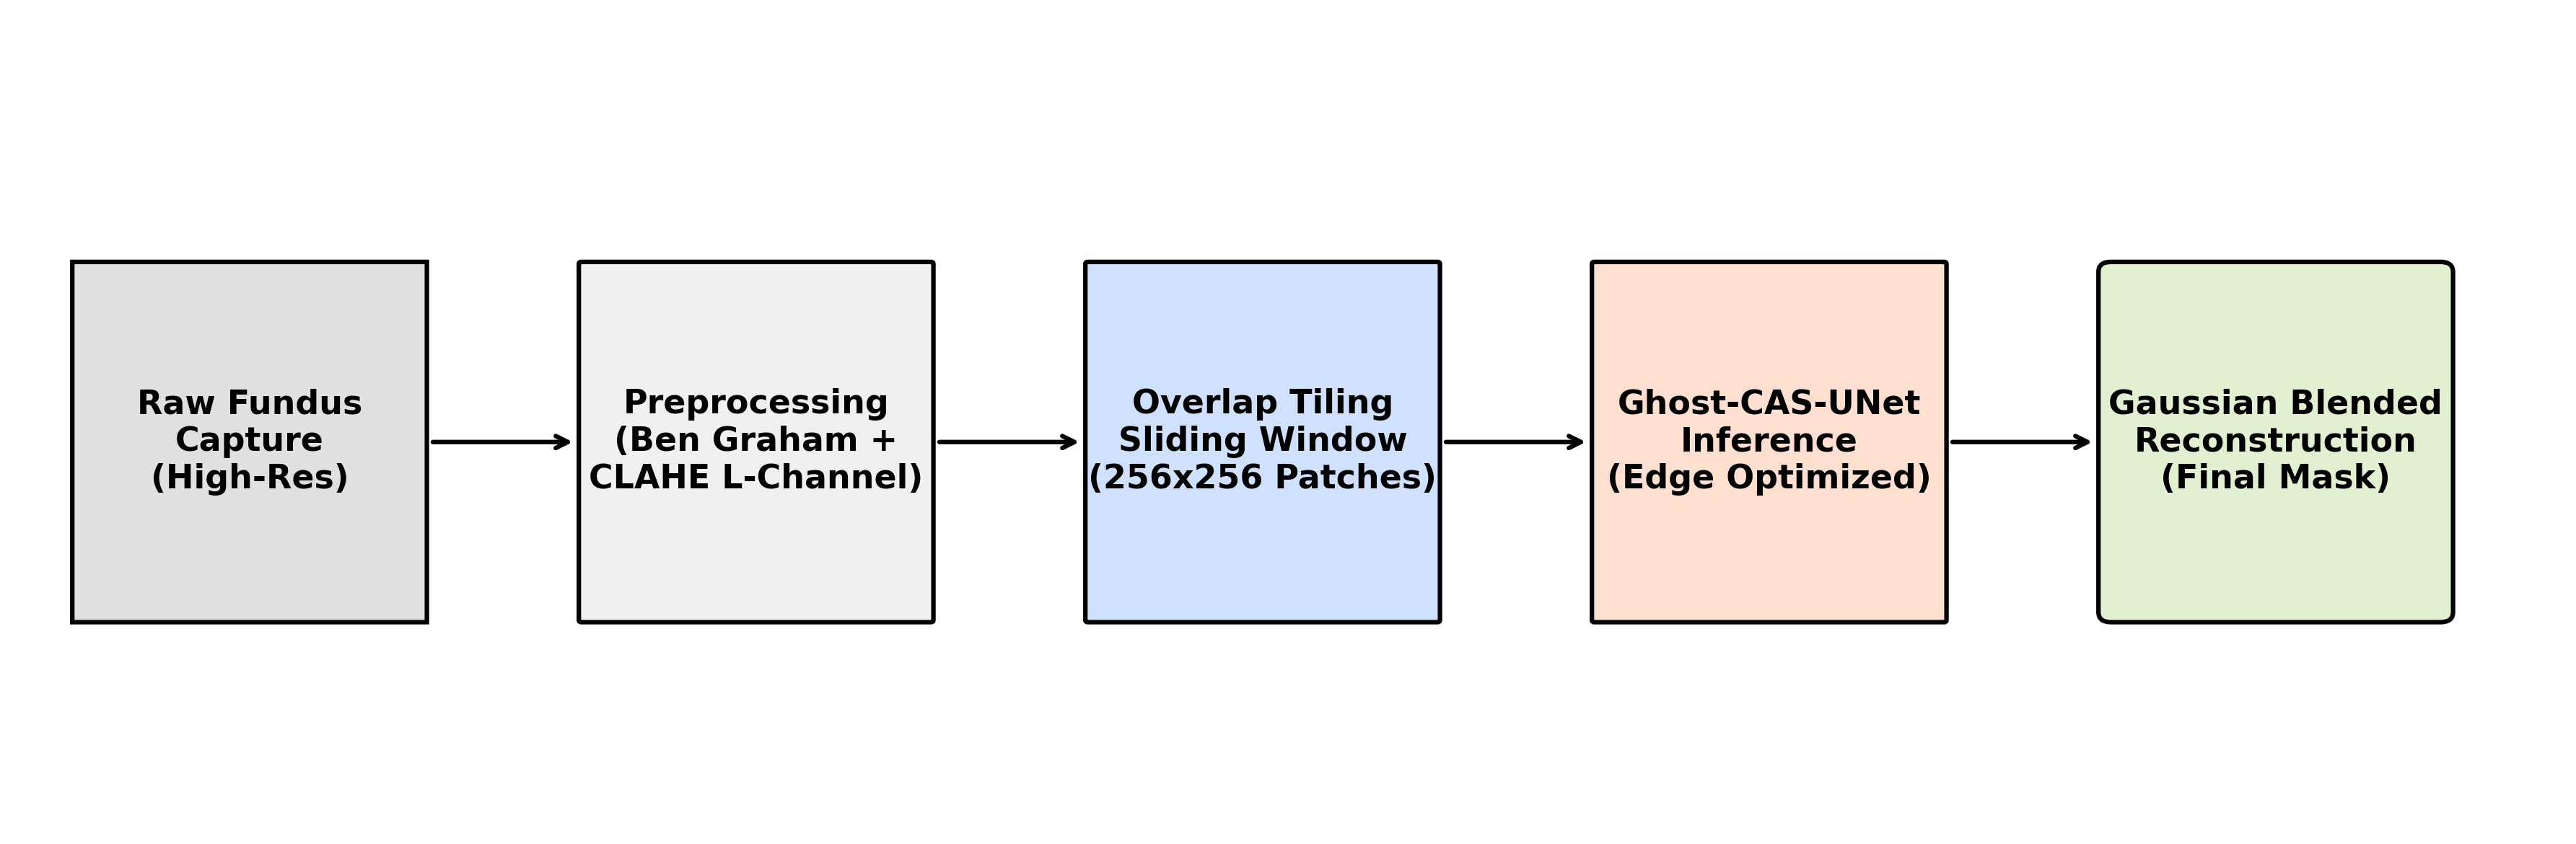
\includegraphics[width=\columnwidth]{images/pipeline_methodology.png}}
\caption{Proposed real-world edge-deployable pipeline: Retinal image capture $\rightarrow$ Preprocessing $\rightarrow$ Sliding window extraction ($256 \times 256$) $\rightarrow$ Model Inference $\rightarrow$ Output Mask Reconstruction via Gaussian Blending.}
\label{fig:pipeline}
\end{figure}

\subsection{Retinal Preprocessing}
Consistent illumination is critically lacking in raw fundus captures, often obscuring low-contrast lesions (MAs/HEs). The foundational step of our pipeline applies Ben Graham Normalization \cite{ben_graham_2015}, wherein a broad Gaussian blur (sigma scaled corresponding to image dimensions) is subtracted from the original RGB distribution. This explicitly suppresses illumination transients triggered by the fundus camera apparatus.

Following normalization, local topological enhancements are achieved via Contrast Limited Adaptive Histogram Equalization (CLAHE). Based on recent improvements in IDRiD challenge pipelines \cite{canet_2020, semi_sup_aaai_2021}, to prevent chrominance distortion when amplifying features, the image is shifted into the LAB colour space, constraining histogram equalization uniquely over the L (Luminance) channel. Finally, a Field-of-View (FOV) morphological mask—computed through thresholding and morphological closing operations—is applied to eliminate pure background sampling waste during the initial data generation.

\subsection{Architecture Design: Ghost-CAS-UNet}
The proposed segmentation backbone, Ghost-CAS-UNet (illustrated in Fig. \ref{fig:architecture}), heavily amends traditional architectures to prioritize inference swiftness concurrently preserving precision. Let the input fundus patch be defined as \(\mathbf{x} \in \mathbb{R}^{H \times W \times 3}\). The network ultimately produces dense class logits \(\mathbf{z} \in \mathbb{R}^{H \times W \times C}\), where \(C=5\) represents the targeted pathological structures and background. The final discrete prediction map \(\mathbf{\hat{y}}\) is extracted via pixel-wise channel maximization: \(\mathbf{\hat{y}}_{i,j} = \text{argmax}_c (\text{softmax}(\mathbf{z}_{i,j,c}))\).

\begin{enumerate}
    \item \textbf{Ghost Bottlenecks:} Conventional stacked convolutions are substituted with Ghost Modules \cite{ghostnet_2020}. Let \(\mathbf{X} \in \mathbb{R}^{H' \times W' \times c}\) be input features. The module first generates intrinsic features \(\mathbf{Y}' = \mathbf{X} * \mathbf{f}\) via a primary convolution \(\mathbf{f}\), followed by cheap linear depthwise operations \(\Phi\) to yield \(\mathbf{Y} = [\mathbf{Y}', \Phi(\mathbf{Y}')]\). This drastically strips Floating Point Operations (FLOPs) without losing spatial hierarchy. 
    \item \textbf{Coordinate Attention (CA) Bottleneck:} Minute MAs are highly subject to positional shifts. We fuse Coordinate Attention \cite{coord_attn_2021} adjacent to our Depthwise ASPP bottleneck. For intermediate features \(\mathbf{F} \in \mathbb{R}^{H \times W \times C}\), 1D global pooling is executed along the X and Y axes independently, yielding directional feature vectors. These are concatenated, transformed via a shared \(1 \times 1\) convolution, split, and passed through a Sigmoid activation \(\sigma\) to produce attention weights \(\mathbf{g}^x\) and \(\mathbf{g}^y\). The spatially refined output is therefore:
    \begin{equation}
    \mathbf{\tilde{F}}_{c}(i,j) = \mathbf{F}_{c}(i,j) \times \mathbf{g}^x_{c}(i) \times \mathbf{g}^y_{c}(j)
    \end{equation}
    \item \textbf{Attention Gated Skips \& Output:} Skip connections pass through Attention Gates \cite{attention_unet_2018} selectively filtering activations. Decentralized \(3 \times 3\) prediction heads uncouple the multi-class interference.
\end{enumerate}

To balance minority pathological pixels against the overwhelming healthy background, the network is optimized using a hybrid objective function \(\mathcal{L}_{Total}\) combining uniform Focal Loss (\(\mathcal{L}_{Focal}\)) and structural Dice Loss (\(\mathcal{L}_{Dice}\)):
\begin{equation}
\mathcal{L}_{Focal} = - \frac{1}{N} \sum_{i=1}^{N} \alpha_{c} (1 - p_{i,c})^\gamma \log(p_{i,c})
\end{equation}
\begin{equation}
\mathcal{L}_{Dice} = 1 - \frac{2 \sum_{i} y_i p_i + \epsilon}{\sum_{i} y_i + \sum_{i} p_i + \epsilon}
\end{equation}
where \(p_{i,c} = \text{softmax}(\mathbf{z}_{i,c})\), \(\alpha_c\) balances class weights, and \(\gamma=2\) heavily penalizes confident misclassifications. Weight decay (\(\lambda = 10^{-5}\)) is appended as an \(L_2\) regularization constraint.

\begin{figure}[htbp]
\centerline{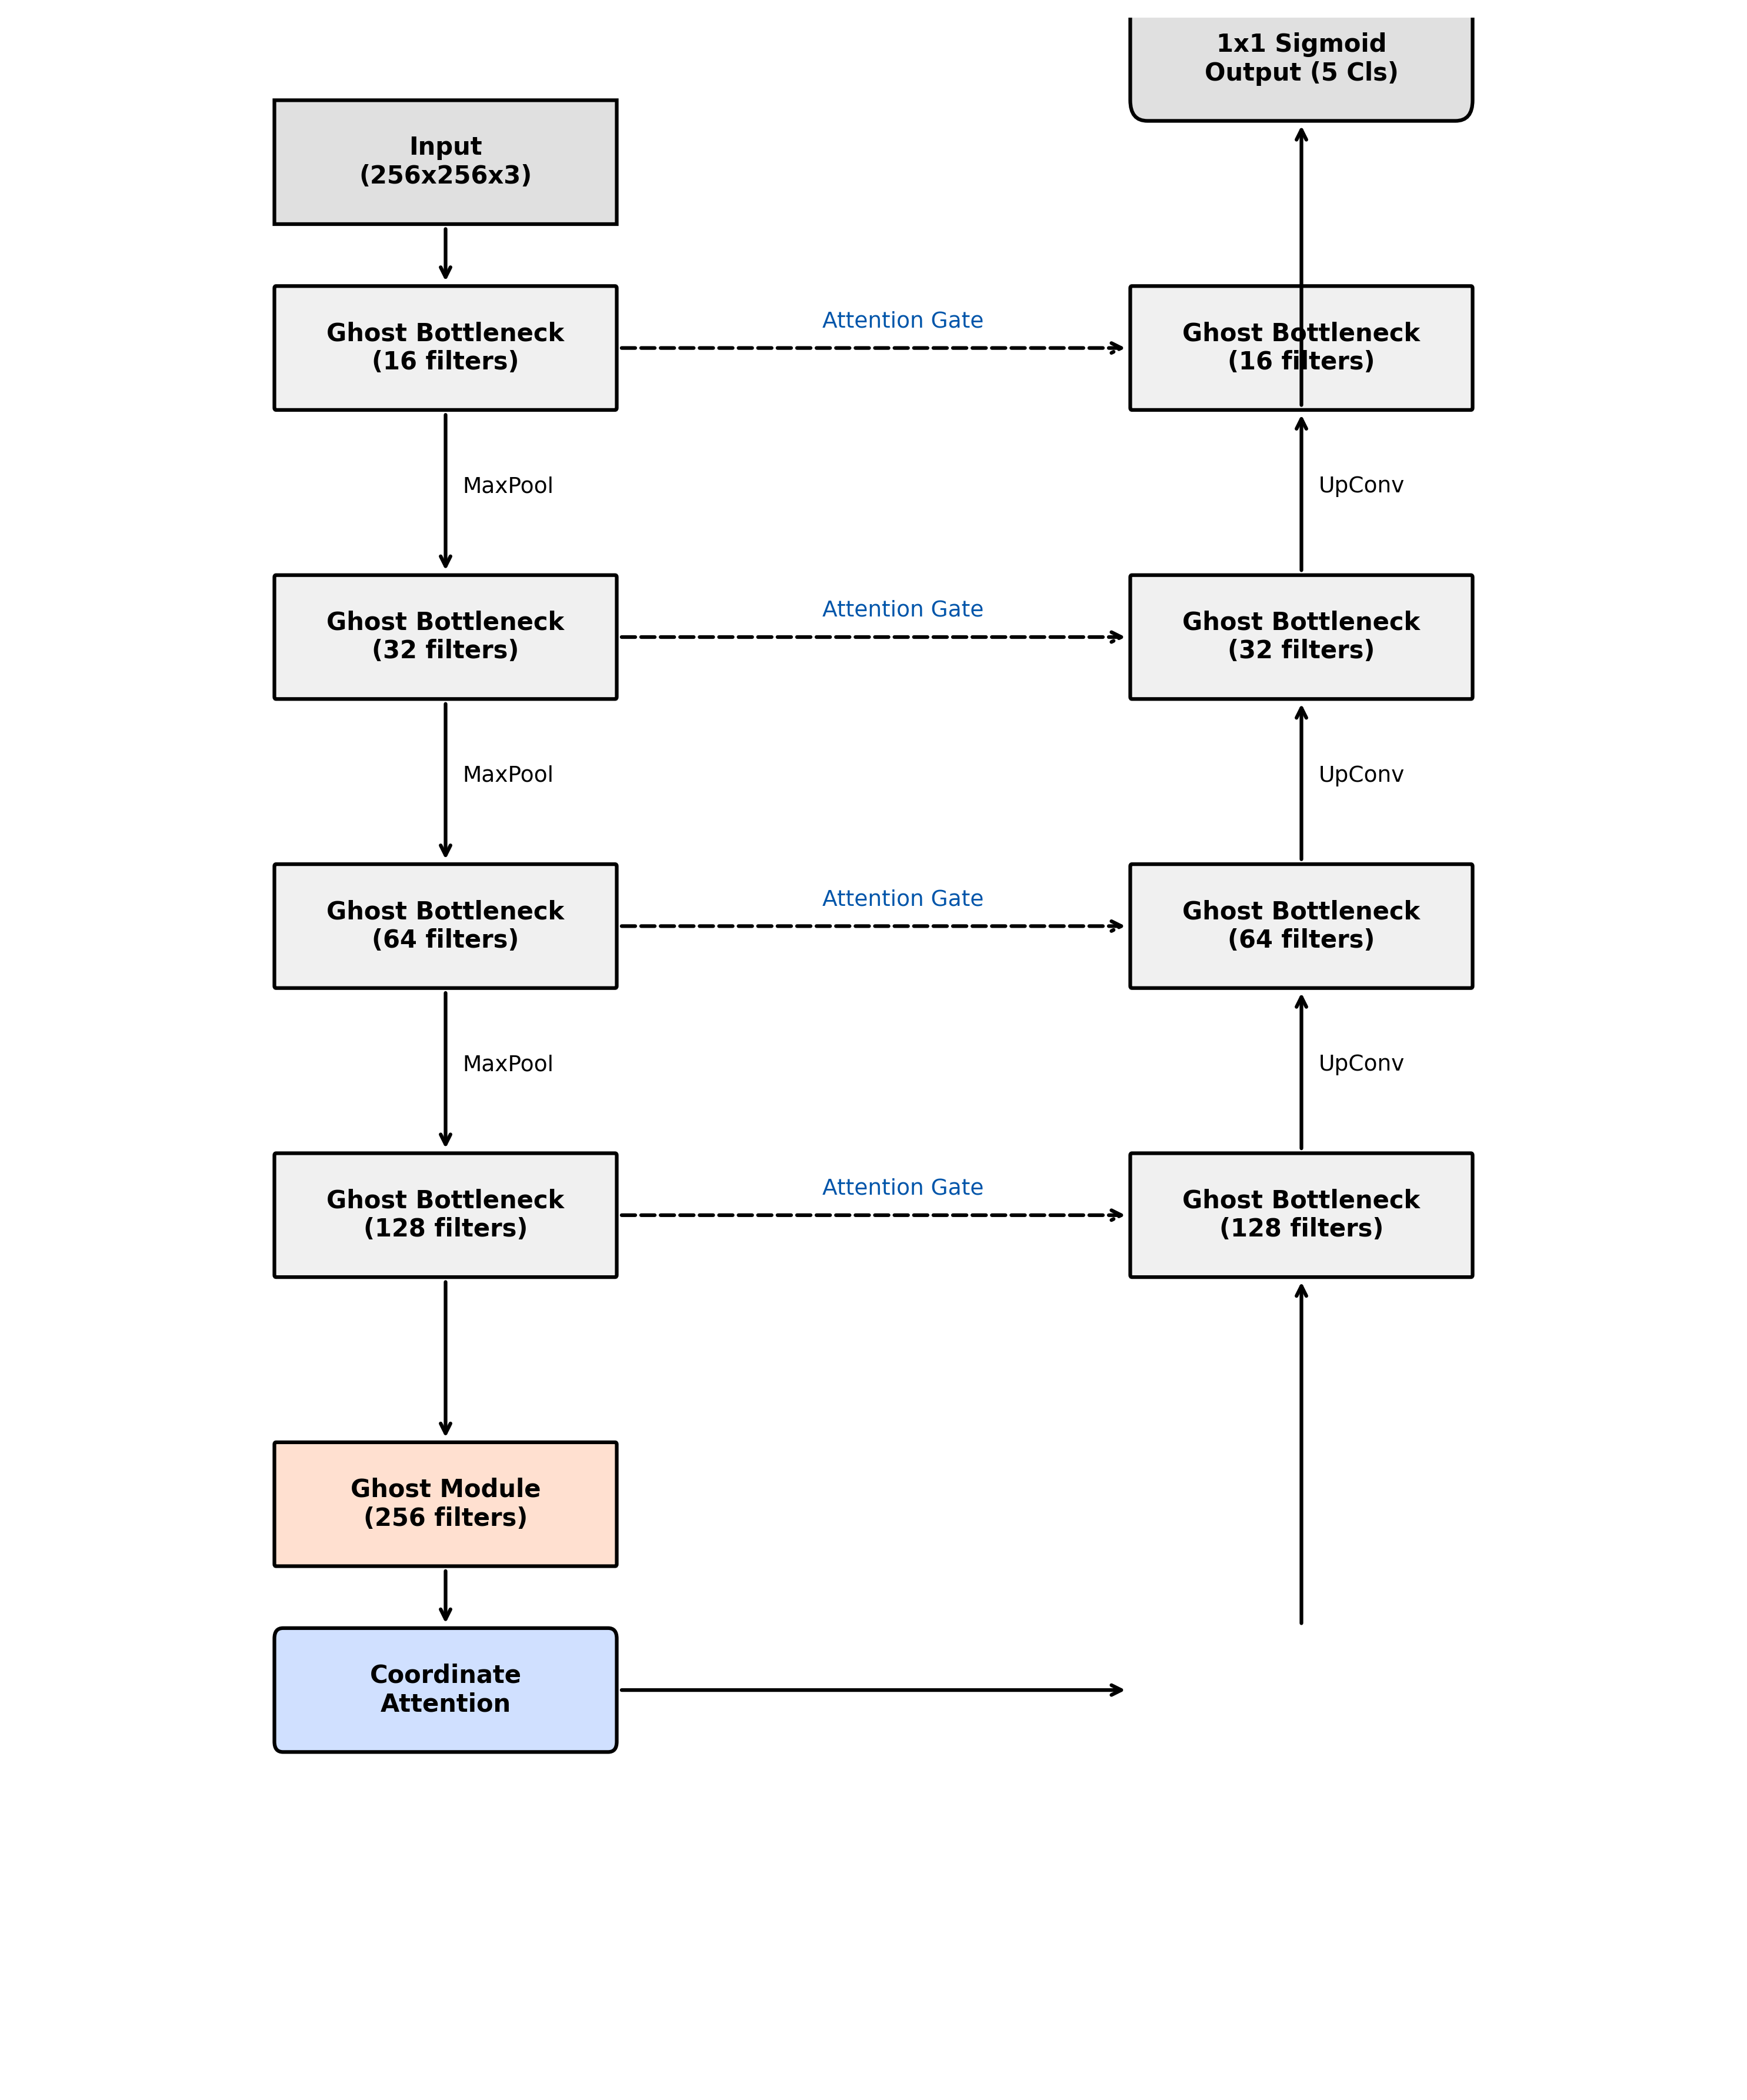
\includegraphics[width=\columnwidth]{images/architecture_ghost_cas.png}}
\caption{Proposed Ghost-CAS-UNet block diagram. The unified architecture pairs linear Depthwise Ghost Bottlenecks for spatial feature economy with exact Cartesian Coordinate Attention resolving minute microaneurysms.}
\label{fig:architecture}
\end{figure}

\subsection{Hyperparameters and Training Strategy}
To balance high resolution feature extraction against VRAM constraints required for edge deployment, we constrained the model to train and infer strictly on $256 \times 256$ spatial patches. This critical architectural decision significantly lowers the peak memory ceiling, ensuring reliable deployment on edge computing modules. Output predictions are seamlessly merged via an overlap-tile strategy mapped with a Gaussian weighting to eliminate boundary seam transients.

Deep supervision was instituted by spawning auxiliary heads at earlier decoder planes, smoothing gradient propagation. Overall parameterization relied firmly on the details specified in Table \ref{tab:hyperparams}.

\begin{table}[htbp]
\caption{Implementation Details and Hyperparameters}
\begin{center}
\begin{tabular}{|l|l|}
\hline
\textbf{Parameter} & \textbf{Value} \\
\hline
Input Resolution & $512 \times 512$ \\
Patch Size (Training) & $256 \times 256$ \\
Batch Size & 16 \\
Optimizer & AdamW \\
Initial Learning Rate & $1 \times 10^{-4}$ \\
Weight Decay & $1 \times 10^{-5}$ \\
Loss Function & Dice Loss + Focal Loss \\
Epochs & 100 (Early Stopping at 85) \\
Augmentation & Flips, Rotations, Color Jitter \\
\hline
\end{tabular}
\label{tab:hyperparams}
\end{center}
\end{table}
